{\section{Unity Physik}}
\label{sec:physik}
Unity ermöglicht mit der eingebauten Physikengine weitestgehend realistische Berechnung von Kollisionen, Schwerkraft und weiteren Kräften.



Die Festkörper (Rigidbody) Komponente ermöglicht es 3D Objekte als nicht verformbares Objekt physikalisch zu simulieren.
\begin{figure}[H]
  \centering  
  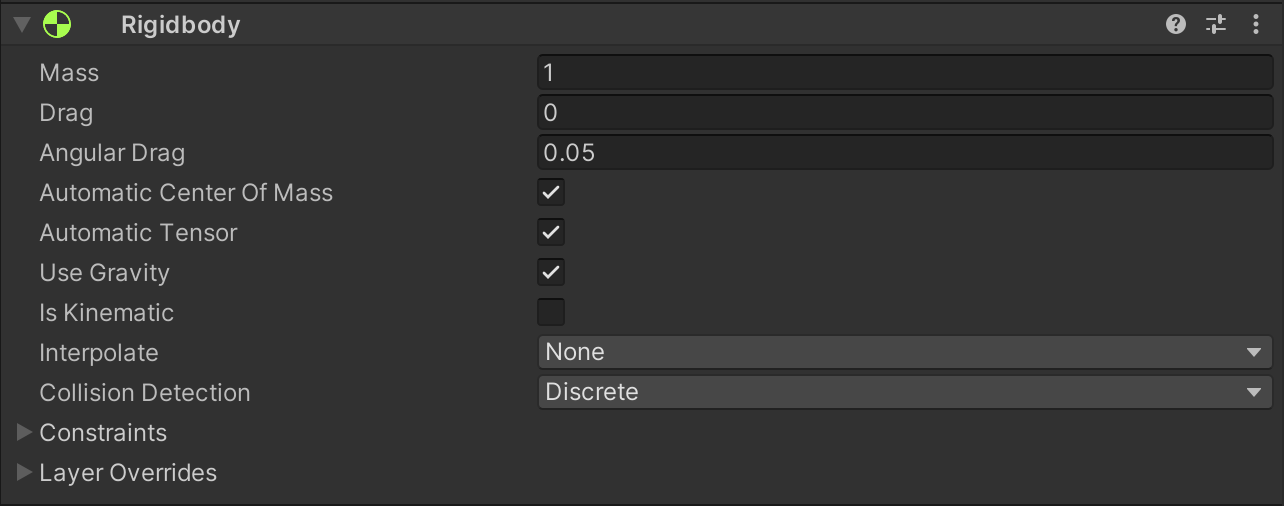
\includegraphics[scale=0.5]{img/physik_festkoerper.png}
  \caption{Unity ML-Agents Physik Festkörper}
  \label{fig:physik_festkoerper}
\end{figure}
\begin{itemize}
  \item Mass: gibt das Gewicht des Körpers an.
  \item Drag: definiert den Geschwindigkeitsverlust eines Körpers in Bewegung durch Reibung, Luftwiederstand
  \item Angular Drag: definiert den Geschwindigkeitsverlust eines Körpers für Rotationsbewegung
  \item Collision Detection: legt fest wie Kollisionen berechnet werden (Akkurat/Leistung)
 \end{itemize}
 
 Um Kollisionen zwischen Objekten zu berechnen benötigen diese zusätzlich eine Kollisionskomponente. Zur Optimierung werden zur Berechnung der Kollisionen die Körper vereinfacht dargestellt. Komplexe 3D Modelle werden als Kugel, Kapsel oder Box vereinfacht.
 \begin{figure}[H]
  \centering  
  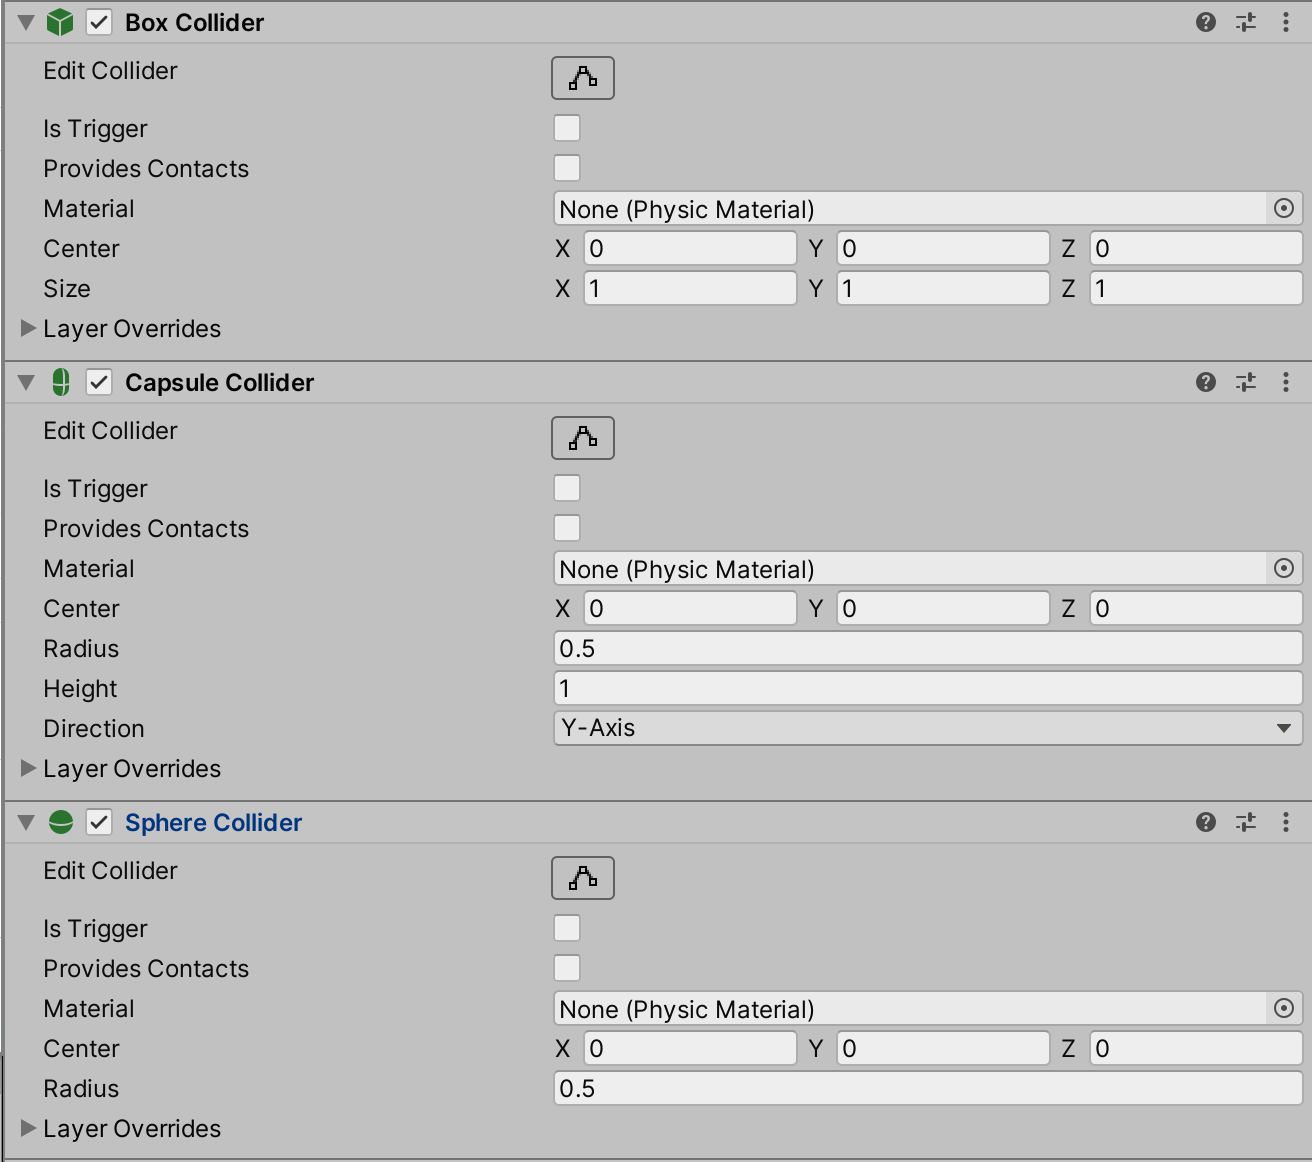
\includegraphics[scale=0.5]{img/physik_kollision.png}
  \caption{Unity ML-Agents Physik Kollisionskomponenten}
  \label{fig:physik_kollision}
\end{figure}

Festkörper können mit Gelenken zu komplexeren Körperstrukturen verbunden werden. Die Konfigurierbare Gelenkkomponente (Configurable Joint) ermöglicht es ein Gelenk mit freier Bewegung und Rotation auf allen 3 Achsen zu simulieren. Im Kontext dieser Arbeit wird das Gelenk dabei auf Rotation beschränkt und als Kugelförmiges Gelenk verwendet.
\begin{figure}[H]
  \centering  
  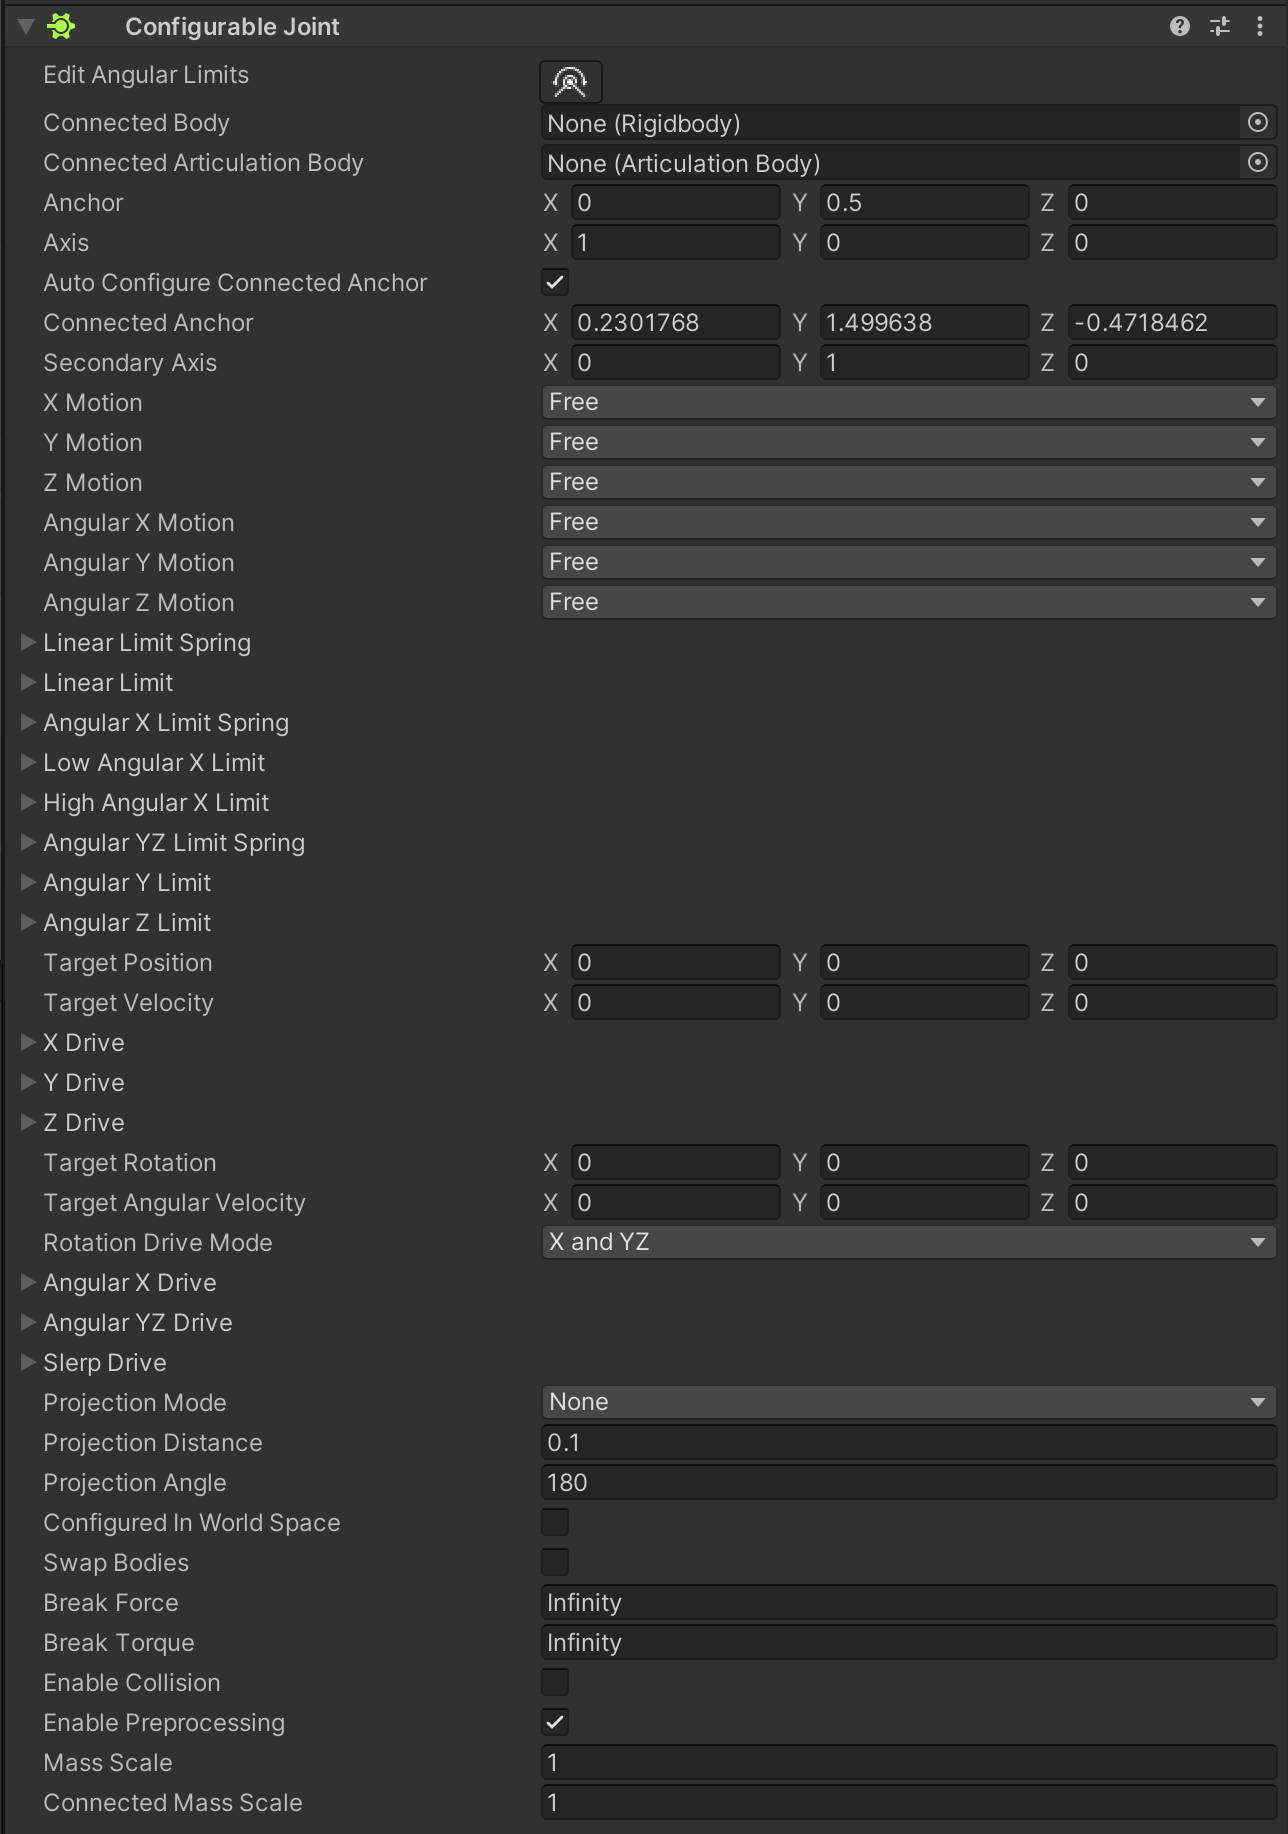
\includegraphics[scale=0.5]{img/physik_gelenk.png}
  \caption{Unity ML-Agents Physik Gelenk}
  \label{fig:physik_gelenk}
\end{figure}
\begin{itemize}
  \item Connected Body: bestimmt mit welchem Körper das Gelenke verbunden ist
  \item Anchor: legt fest an welchem Punkt die Verbindung zum verbundenen Körper besteht
  \item Axis: legt die Hauptbewegungs- und Rotationsachse fest
  \item Secondary Axis: legt die sekundäre Beweungs- Rotationsachse fest
  \item Angular X Y Z Motion: bestimmt ob das Gelenk Rotation zwischen den Körpern auf der X Y Z Achse zulässt
  \item Target Position: bestimmt das Ziel zu welchem das Gelenk sich bewegen soll
  \item Angular X Y Z Limit: ermöglicht das festlegen von Winkellimits für die Rotationsbewegungen
  \item X Y Z  und Slerp Drive: bestimmen die Stärke der Federkraft welche das Gelenk in die Zielposition bewegt
\end{itemize}